% filepath: /home/liutao/Desktop/homework/hello_world.tex
\documentclass{article}
\usepackage{CJKutf8}
\usepackage{listings}
\usepackage{graphicx}
\usepackage{float} 
\begin{document}
\begin{CJK}{UTF8}{gbsn}
\title{HPC 大作业}
\author{刘涛}
\date{\today}

\maketitle

\section{第一题}
\subsection{编译CloverLeaf}
1.Serial 版本的CloverLeaf\\
观察Serial文件下的README.MD文件可以知道使用
\begin{lstlisting}[language=C++]
    make COMPILER=GNU MPI_COMPILER=gfortran C_MPI_COMPILER=gcc
\end{lstlisting} 
编译运行指令,如下所示:
\begin{figure}[H]
    \centering
    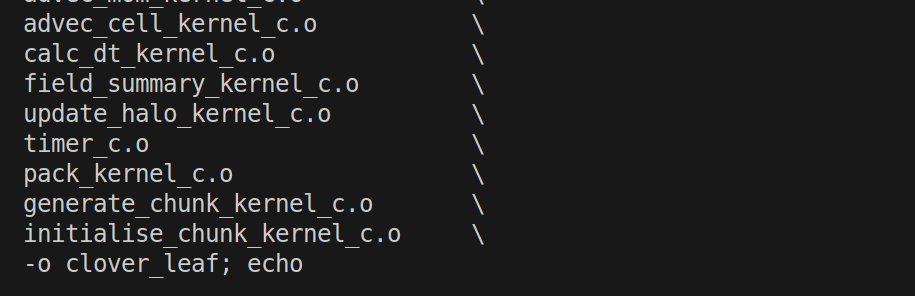
\includegraphics[width=0.8\textwidth]{./serial2.png}
    \caption{Serial 版本编译结果}
\end{figure} 

直接运行的结果,如下所示:
\begin{figure}[H]
    \centering
    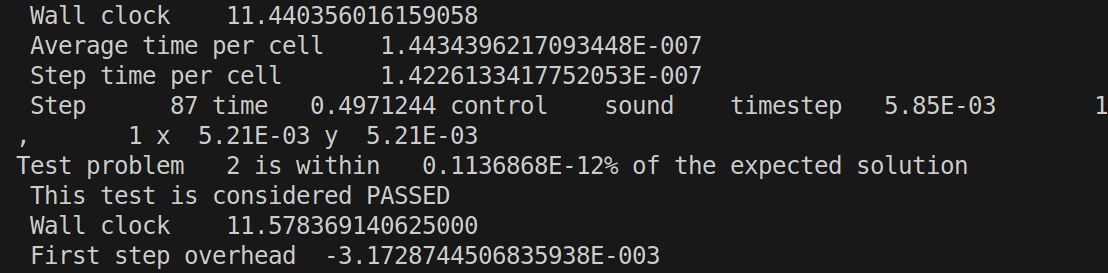
\includegraphics[width=0.8\textwidth]{./serial1.png}
    \caption{Serial 版本运行结果}
\end{figure} 

2.MPI 版本的CloverLeaf
同理,观察README.MD文件,由于我使用的是GNU编译器,可知采用
\begin{lstlisting}[language=C++]
make COMPILER=GNU MPI_COMPILER=mpifort C_MPI_COMPILER=mpicc DEBUG=1 IEEE=1
\end{lstlisting} 
编译运行指令,如下所示:
\begin{figure}[H]
    \centering
    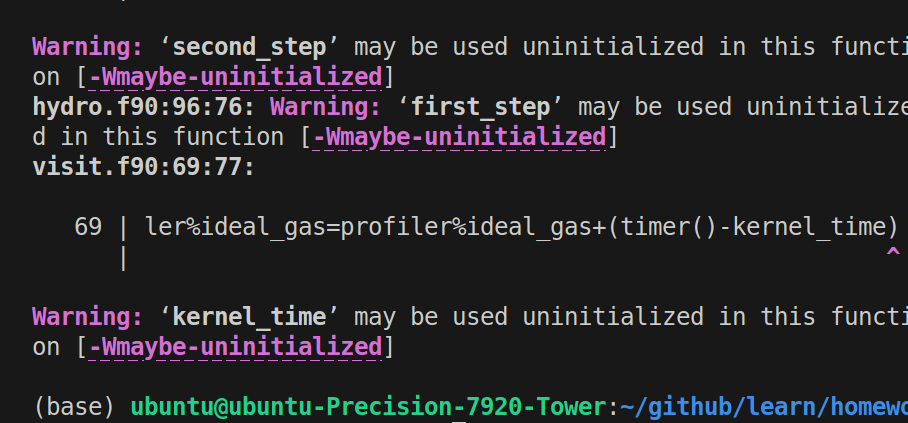
\includegraphics[width=0.8\textwidth]{./MPI1.png}
    \caption{MPI 版本编译结果}
\end{figure} 

直接运行的结果,如图片4所示:
\begin{figure}[H]
    \centering
    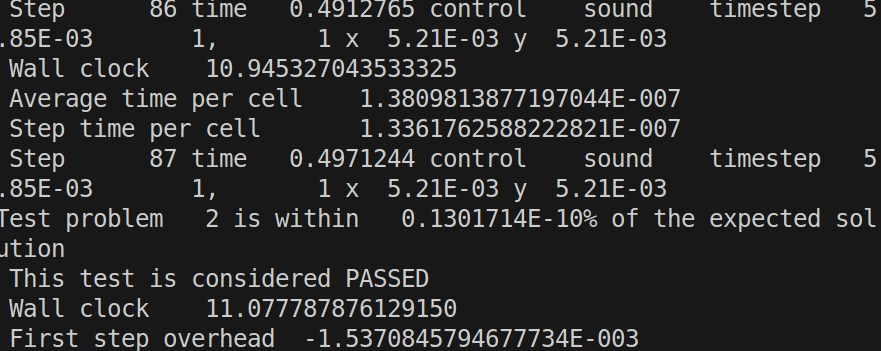
\includegraphics[width=0.8\textwidth]{./MPI2.png}
    \caption{MPI 版本运行结果}
\end{figure}

3. OPENMP版本的ColverLeaf

继续观察openmp的CloverLeafOpenmp下README.md,同样得到采用相同的编译指令运行OPENMP
\begin{lstlisting}[language=C++]
    make COMPILER=GNU MPI_COMPILER=mpifort C_MPI_COMPILER=mpicc DEBUG=1 IEEE=1
\end{lstlisting} 
    编译运行指令,如图片5所示:
    
    \begin{figure}[H]
        \centering
        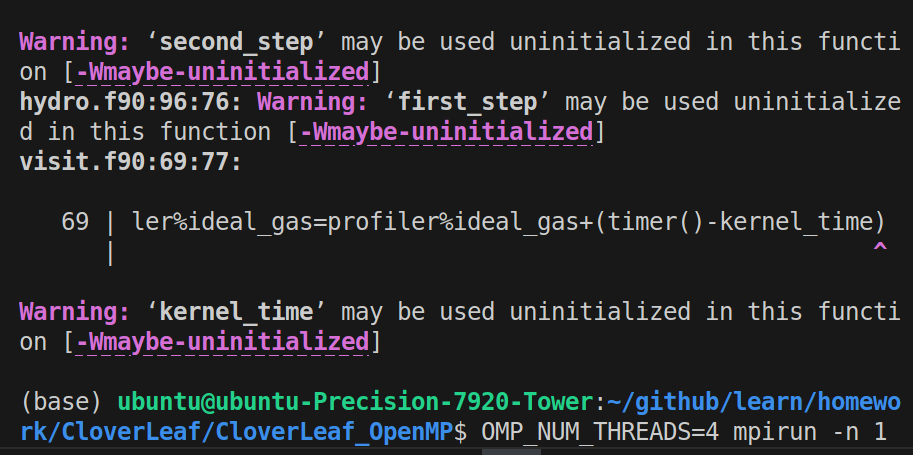
\includegraphics[width=0.8\textwidth]{./OPENMP1.png}
        \caption{OPENMP 版本编译结果}
    \end{figure} 
    
    直接运行的界面,如图片6所示
    \begin{figure}[H]
        \centering
        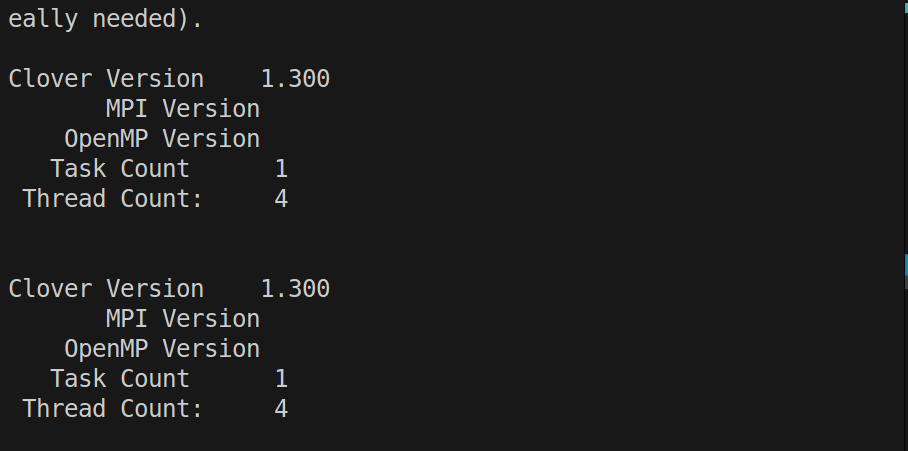
\includegraphics[width=0.8\textwidth]{./OPENMP2.png}
        \caption{OPENMP 版本运行}
    \end{figure}
    
    运行结果,如图片7所示
    \begin{figure}[H]
        \centering
        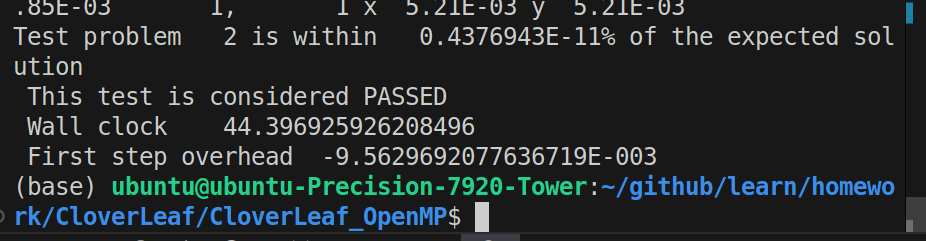
\includegraphics[width=0.8\textwidth]{./OPENMP3.png}
        \caption{OPENMP 版本运行结果}
    \end{figure}

4. MPI+OPENMP版本的ColverLeaf
到这里,结合已经学习的知识和做过的实验,不难验证编译指令如下所示。
\begin{lstlisting}[language=C++]
    make COMPILER=GNU MPI_COMPILER=mpifort C_MPI_COMPILER=mpicc DEBUG=1 IEEE=1
\end{lstlisting} 
\begin{lstlisting}[language=C++]
    OMP_NUM_THREAD=4 mpirun -n 4 ./clover_leaf
\end{lstlisting} 
测试结果如图片8所示:
\begin{figure}[H]
    \centering
    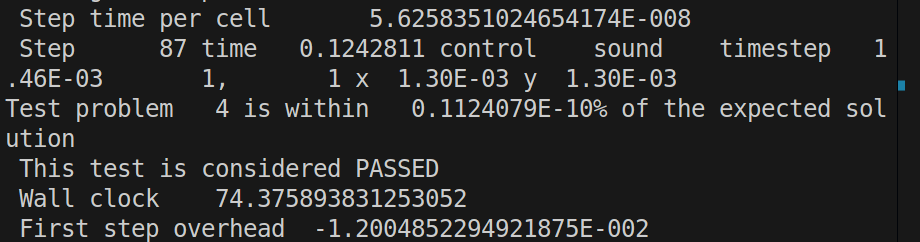
\includegraphics[width=0.8\textwidth]{./ref1.png}
    \caption{MPI+openmp 版本运行结果}
\end{figure}
\subsection{性能分析}
性能分析工具采用intel OneAPI vtune进行处理,这是一款性能优良适合分析的工具。 \\
1.Serial 版本的CloverLeaf性能分析 \\
使用性能分析参数
\begin{lstlisting}[language=C++]
    OMP_NUM_THREAD=1 mpirun -n 1 ./clover_leaf
\end{lstlisting} 
\begin{figure}[H]
    \centering
    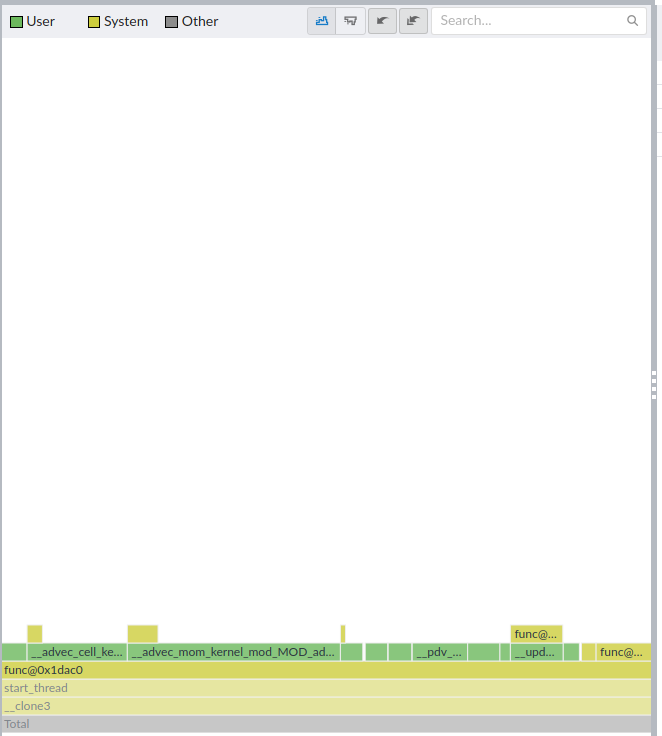
\includegraphics[width=0.8\textwidth]{./call1.png}
    \caption{Serial 版本运行火焰图}
\end{figure}

采用Bottomup的分析模式可以知道程序中的热点位置在于 \\
\begin{figure}[H]
    \centering
    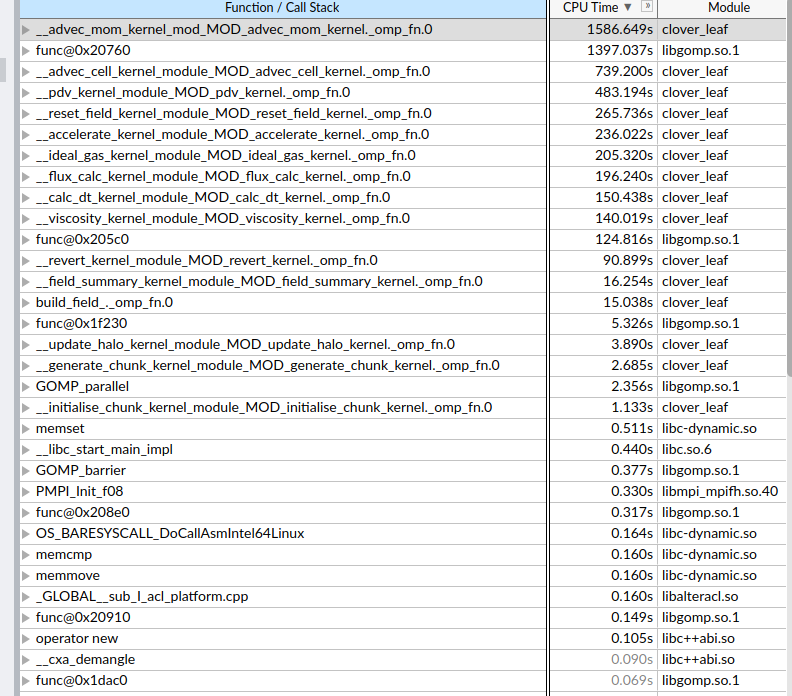
\includegraphics[width=0.8\textwidth]{./call2.png}
    \caption{Serial 版本运行热点图}
\end{figure}
由于Serial版本的代码不支持重定位到具体的代码细节,详细的分析在后续写下.\\
2.MPI 版本的CloverLeaf性能分析
采用如下版本进行分析\\
\begin{lstlisting}[language=C++]
    OMP_NUM_THREAD=1 mpirun -n 4 ./clover_leaf
\end{lstlisting} 
\begin{figure}[H]
    \centering
    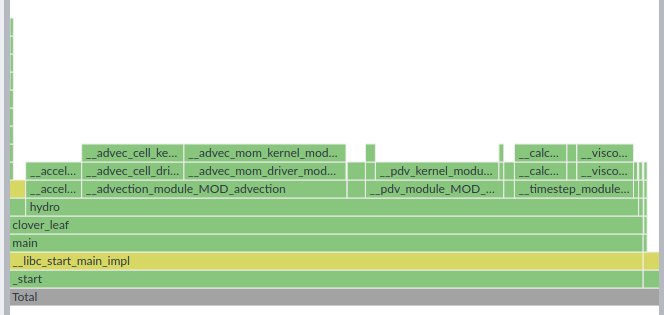
\includegraphics[width=0.8\textwidth]{./call3.png}
    \caption{MPI 版本运行火焰图}
\end{figure}
采用Bottomup的分析模式可以知道程序中的热点位置在于 \\
\begin{figure}[H]
    \centering
    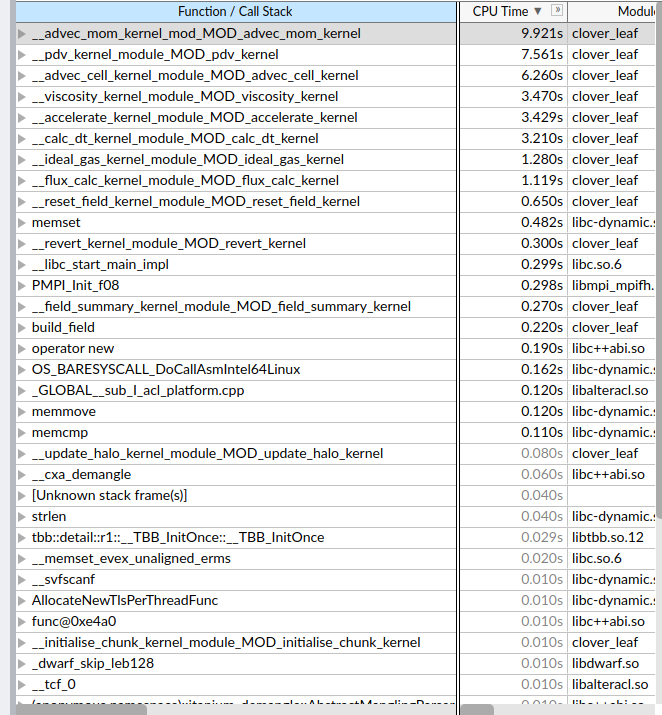
\includegraphics[width=0.8\textwidth]{./call4.png}
    \caption{MPI 版本运行热点图}
\end{figure}
对于在Bottomup图中的消耗CPU时间最多的函数,其代码如下所示\\
\begin{figure}[H]
    \centering
    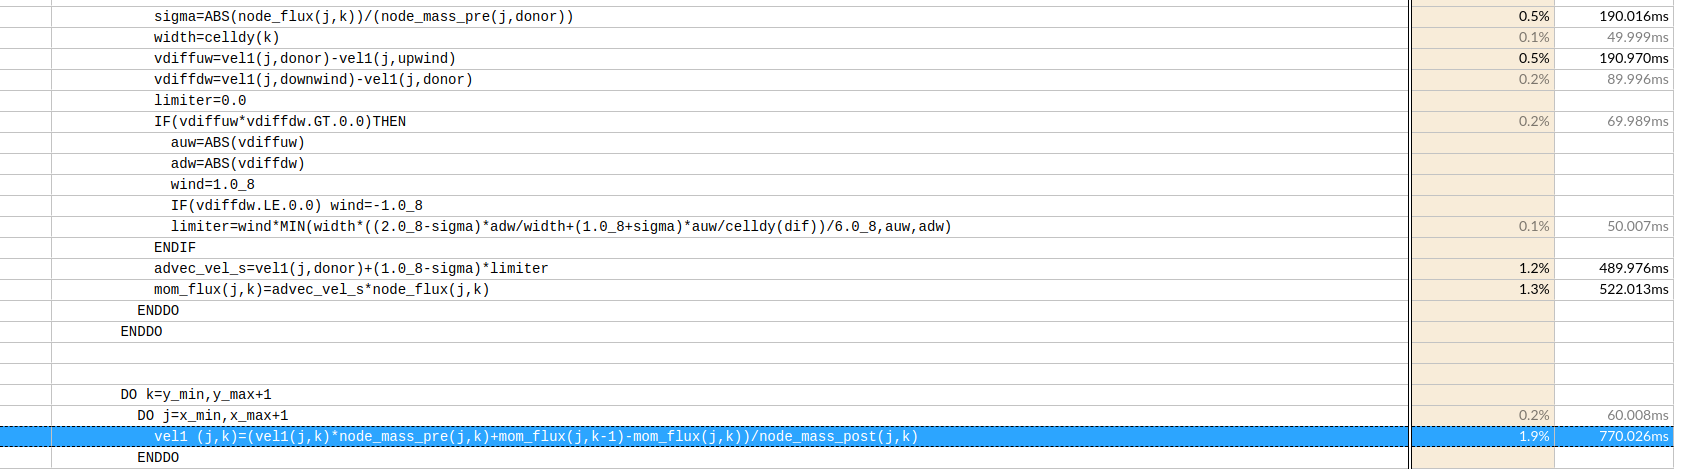
\includegraphics[width=0.8\textwidth]{./call5.png}
    \caption{源码所在函数}
\end{figure}
\begin{figure}[H]
    \centering
    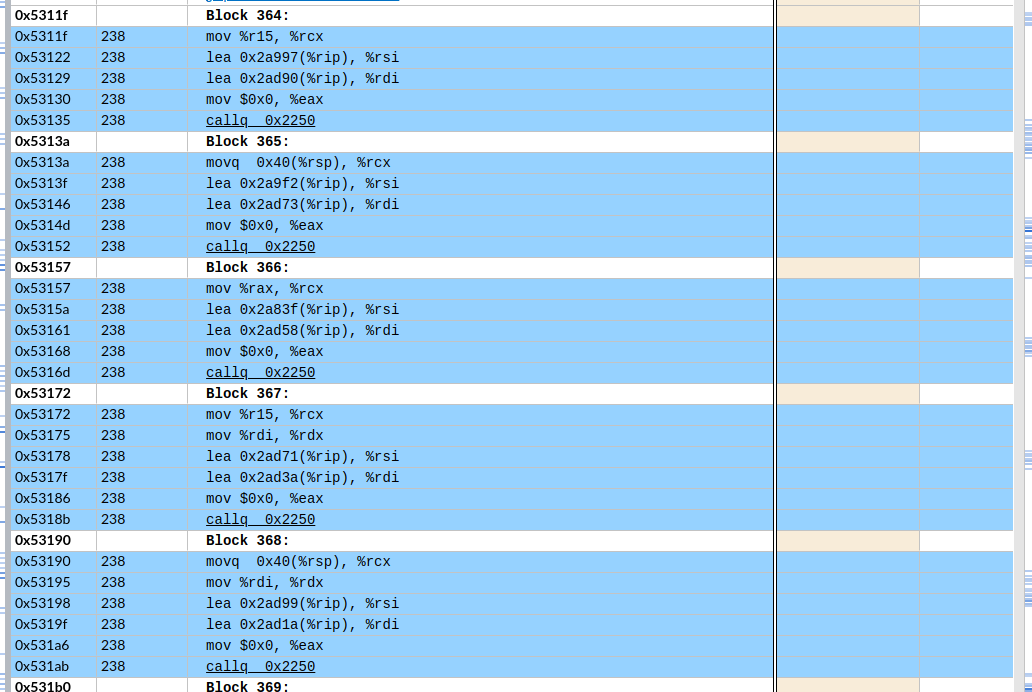
\includegraphics[width=0.8\textwidth]{./call6.png}
    \caption{反汇编图片}
\end{figure}

3.OPENMP 版本的CloverLeaf性能分析
\begin{lstlisting}[language=C++]
    OMP_NUM_THREAD=4 mpirun -n 1 ./clover_leaf
\end{lstlisting} 
\begin{figure}[H]
    \centering
    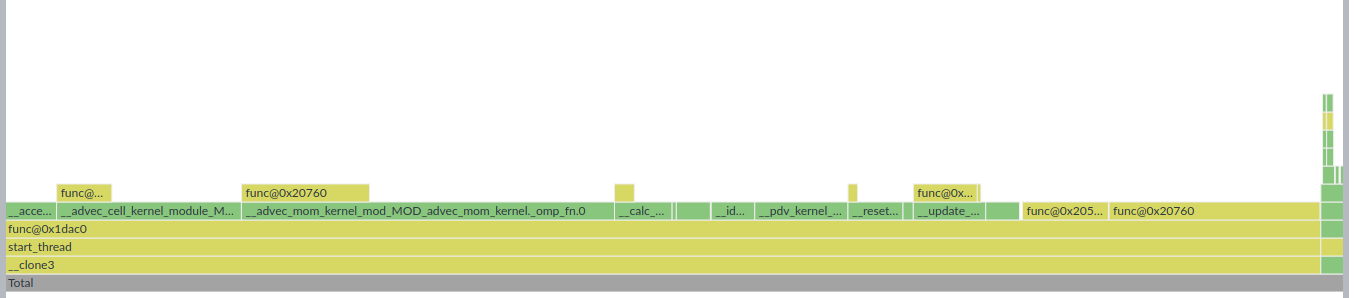
\includegraphics[width=0.8\textwidth]{./call7.png}
    \caption{OPENMP 版本运行火焰图}
\end{figure}
采用Bottomup的分析模式可以知道程序中的热点位置在于 \\
\begin{figure}[H]
    \centering
    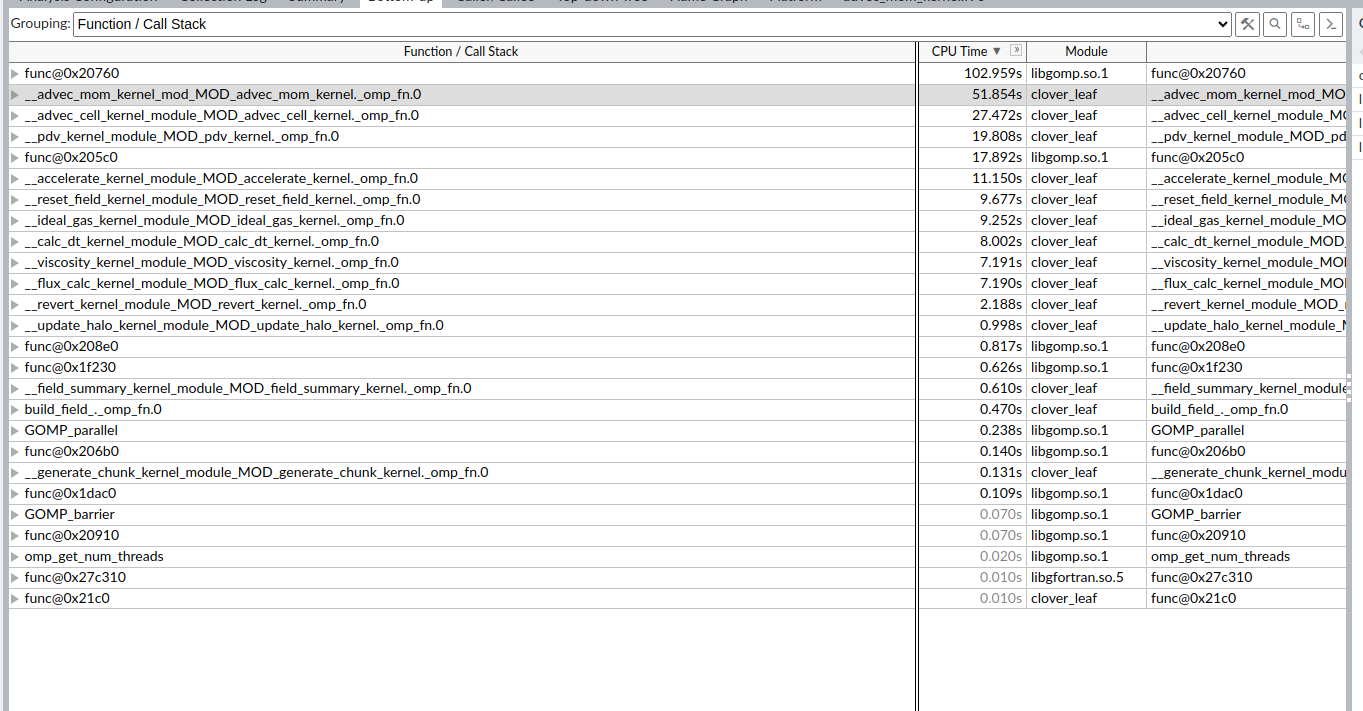
\includegraphics[width=0.8\textwidth]{./call8.png}
    \caption{OPENMP 版本运行热点图}
\end{figure}
此时再进行分析可知出现了系统函数调用func@0x20760,这说明在这个位置调用了OPENMP的系统函数,
反汇编可知这部分的操作没有对应在程序中的代码,在openmp动态链接库文件中被调用,观察其内容,可能
是对应的资源访问互斥锁。 \\
\begin{figure}[H]
    \centering
    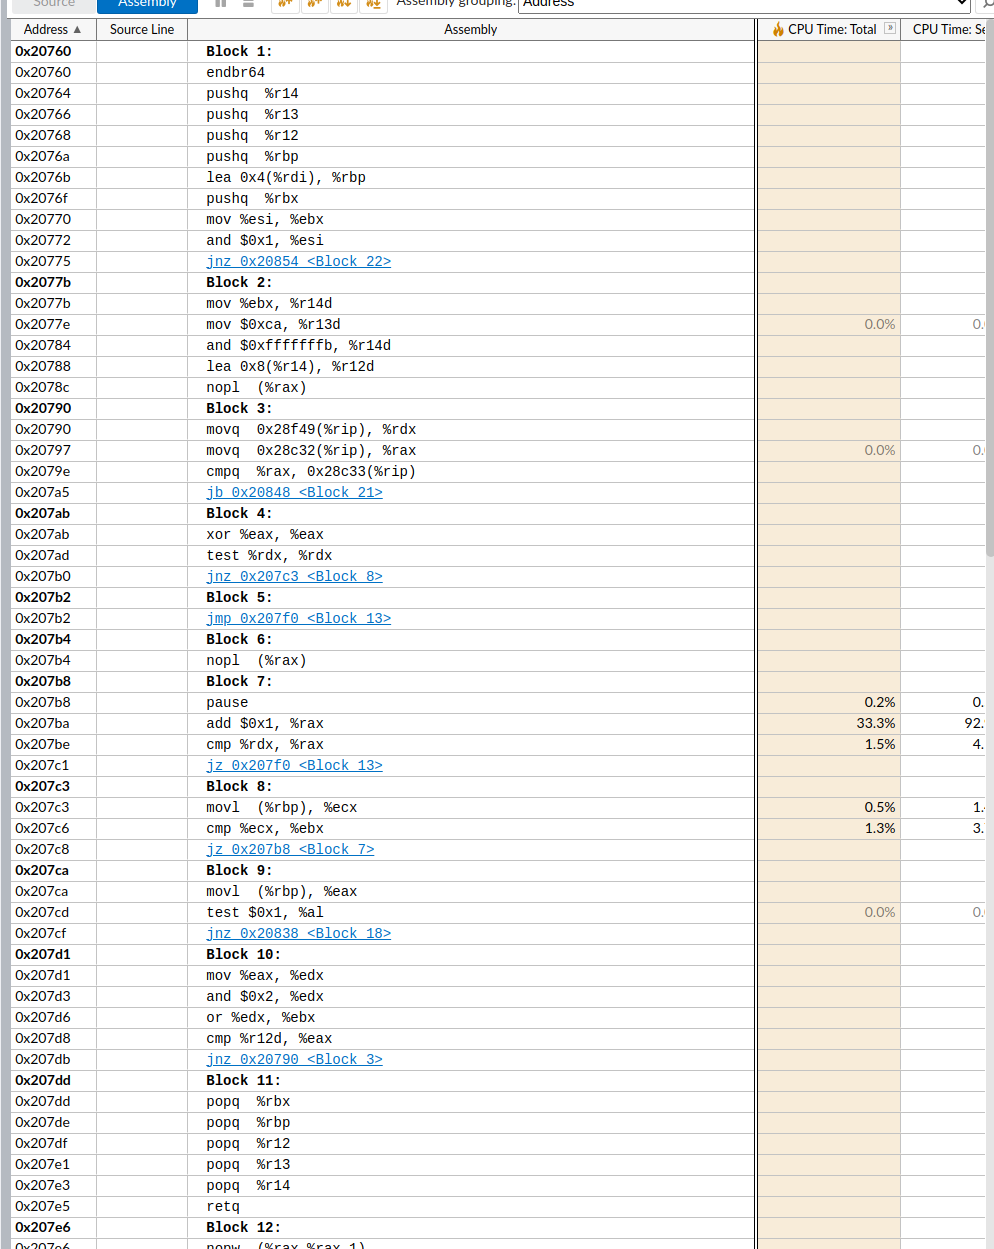
\includegraphics[width=0.8\textwidth]{./call9.png}
    \caption{OPENMP 版本运行热点图}
\end{figure}
4.MPI+OPENMP 版本的CloverLeaf性能分析
\begin{lstlisting}[language=C++]
    OMP_NUM_THREAD=4 mpirun -n 4 ./clover_leaf
\end{lstlisting} 

\begin{figure}[H]
    \centering
    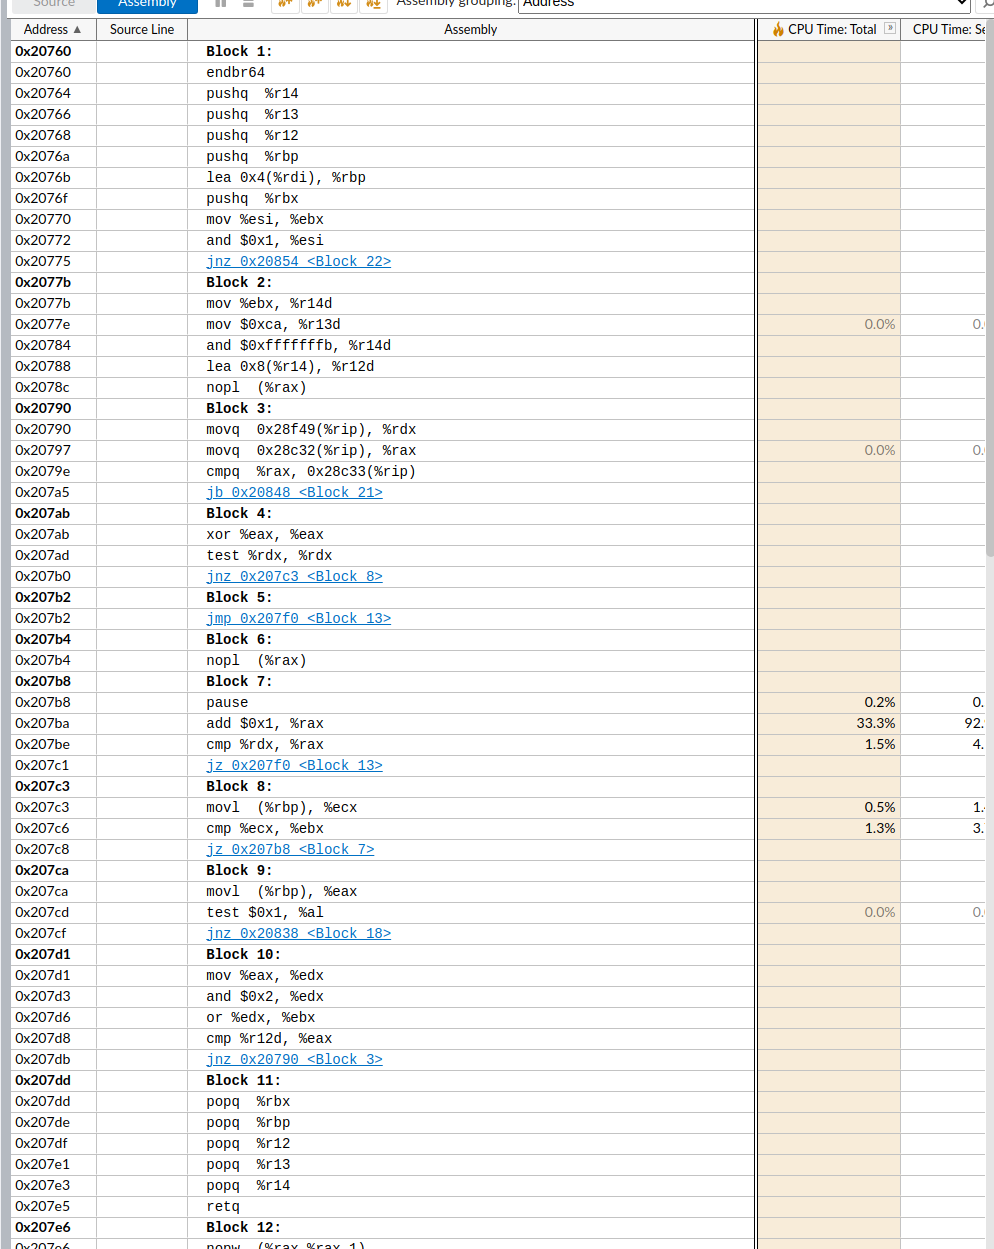
\includegraphics[width=0.8\textwidth]{./call9.png}
    \caption{OPENMP 版本运行热点图}
\end{figure}
\begin{figure}[H]
    \centering
    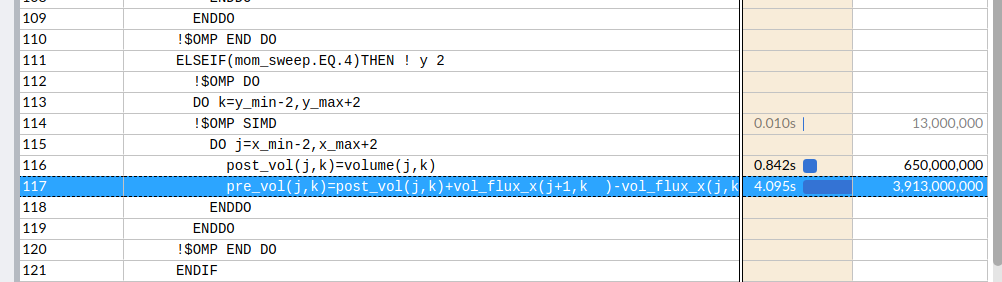
\includegraphics[width=0.8\textwidth]{./call10.png}
    \caption{OPENMP+MPI运行反汇编程序}
\end{figure}
\subsection{效率对比}
1.不同MPI+OPENMP的对比
x\_cell=960,y\_cell=960
\begin{table}[h!]
    \centering
    \begin{tabular}{|c|c|c|}
    \hline
    \textbf{OMP\_NUM\_THREADS} & \textbf{MPI ranks} & \textbf{time consumption} \\
    \hline
    1 & 1 & 47.35715s \\
    \hline
    1 & 2 & 24.93825s \\
    \hline
    1 & 4 & 12.38018s \\
    \hline
    2 & 1 & 43.900086s \\
    \hline
    2 & 2 & 22.80418s \\
    \hline
    2 & 4 & 6.75957 \\
    \hline
    4 & 1 &  44.56657s \\
    \hline
    4 & 2 &  23.21618s \\
    \hline
    4 & 4 &  4.126149s \\
    \hline
    \end{tabular}
    \caption{ref下不同OMP\_NUM\_THREADS and MPI 的时间消耗}
    \label{table:combinations}
\end{table}
\\
x\_cell=1920,y\_cell=1920
\begin{table}[h!]
    \centering
    \begin{tabular}{|c|c|c|}
    \hline
    \textbf{OMP\_NUM\_THREADS} & \textbf{MPI ranks} & \textbf{time consumption} \\
    \hline
    1 & 1 & 188.6974799s \\
    \hline
    1 & 2 & 96.022246s \\
    \hline
    1 & 4 & 49.126179s \\
    \hline
    2 & 2 & 22.80418s \\
    \hline
    2 & 4 & 26.75957 \\
    \hline
    4 & 4 & 19.46512s \\
    \hline
    \end{tabular}
    \caption{ref下不同OMP\_NUM\_THREADS and MPI 的时间消耗}
    \label{table:combinations}
\end{table}
\\
2.不同MPI的对比
\newline
xcell=960,ycell=960
\begin{table}[H]
    \centering
    \begin{tabular}{|c|c|c|}
    \hline
    \textbf{OMP\_NUM\_THREADS} & \textbf{MPI ranks} & \textbf{time consumption} \\
    \hline
    1 & 1 &  37.21615s \\
    \hline
    1 & 2 & 19.731973s \\
    \hline
    1 & 4 & 9.932440s \\
    \hline
    1 & 8 & 5.461988s \\
    \hline
    1 & 16 & 3.7412819s \\
    \hline
    \end{tabular}
    \caption{ref下不同OMP\_NUM\_THREADS and MPI 的时间消耗}
    \label{table:combinations}
\end{table}
3.OPEMP版本的对比
\\
xcell=960,ycell=960
\begin{table}[H]
    \centering
    \begin{tabular}{|c|c|c|}
    \hline
    \textbf{OMP\_NUM\_THREADS} & \textbf{MPI ranks} & \textbf{time consumption} \\
    \hline
    1 & 1 & 46.32359s \\
    \hline
    2 & 1 & 24.176760s \\
    \hline
    4 & 1 & 13.139265s \\
    \hline
    8 & 1 & 7.1625220s \\
    \hline
    16 & 1 & 4.6675159s \\
    \hline
    \end{tabular}
    \caption{OPENMP下不同OMP\_NUM\_THREADS and MPI 的时间消耗}
    \label{table:combinations}
\end{table}
\subsection{CUDA 编译}
由于CUDA版本的编译需要适配,做如下的修改,
使用对应的GNU编译器
\begin{figure}[H]
    \centering
    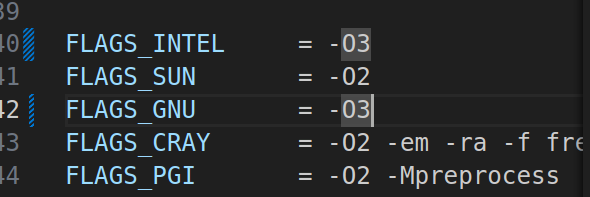
\includegraphics[width=0.8\textwidth]{./compile.png}
    \caption{编译命令修改}
\end{figure}
由于我的fortran版本的是gcc11对应的fortran版本,所以使用对应的编译器会出现早期编译器对浮点数和int类型坚持不严格,而在新编译器上的检查严格造成的错误. 
\begin{figure}[H]
    \centering
    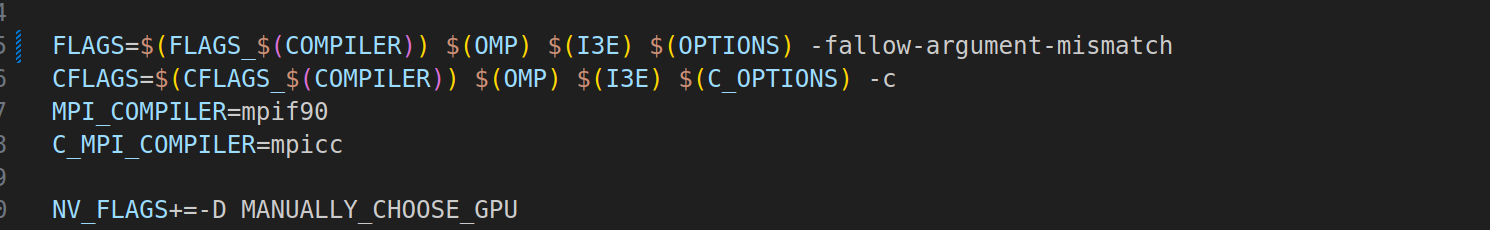
\includegraphics[width=0.8\textwidth]{./compile5.png}
    \caption{编译命令修改}
\end{figure}

\begin{figure}[H]
    \centering
    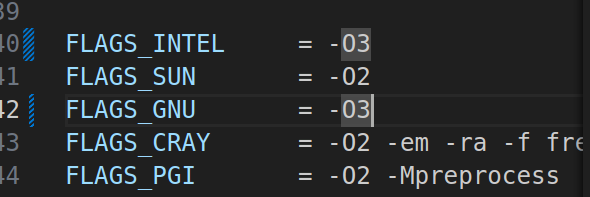
\includegraphics[width=0.8\textwidth]{./compile.png}
    \caption{编译命令修改}
\end{figure}
由于我的电脑是Ampere架构的显卡,修改Makefile文件获得计算结果
\begin{figure}[H]
    \centering
    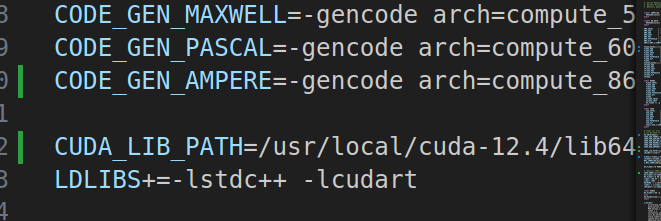
\includegraphics[width=0.8\textwidth]{./compile2.png}
    \caption{修改为Ampere架构}
\end{figure}
CUDA是12.4类型的CUDA,所以修改对应的CUDA编译器
\begin{figure}[H]
    \centering
    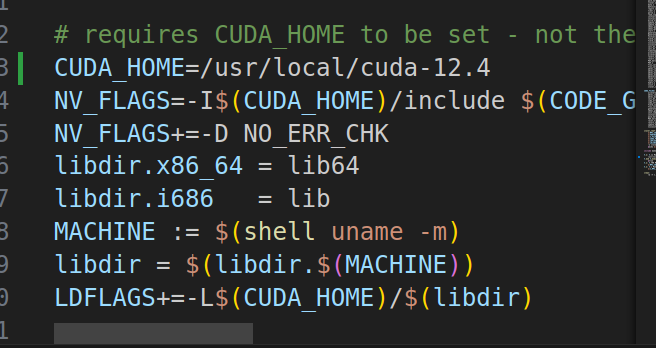
\includegraphics[width=0.8\textwidth]{./com.png}
    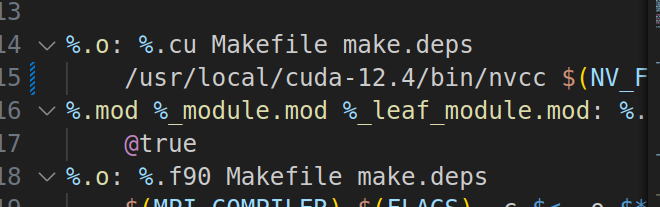
\includegraphics[width=0.8\textwidth]{./compile4.png}
    \caption{指定CUDA和NVCC位置}
\end{figure}
采用如下的编译指令
\begin{lstlisting}[language=C++]
    make COMPILER=GNU MPI_COMPILER=mpifort C_MPI_COMPILER=mpicc DEBUG=1 IEEE=1
\end{lstlisting} 
成功编译对应的程序,其结果如下所示
\begin{figure}[H]
    \centering
    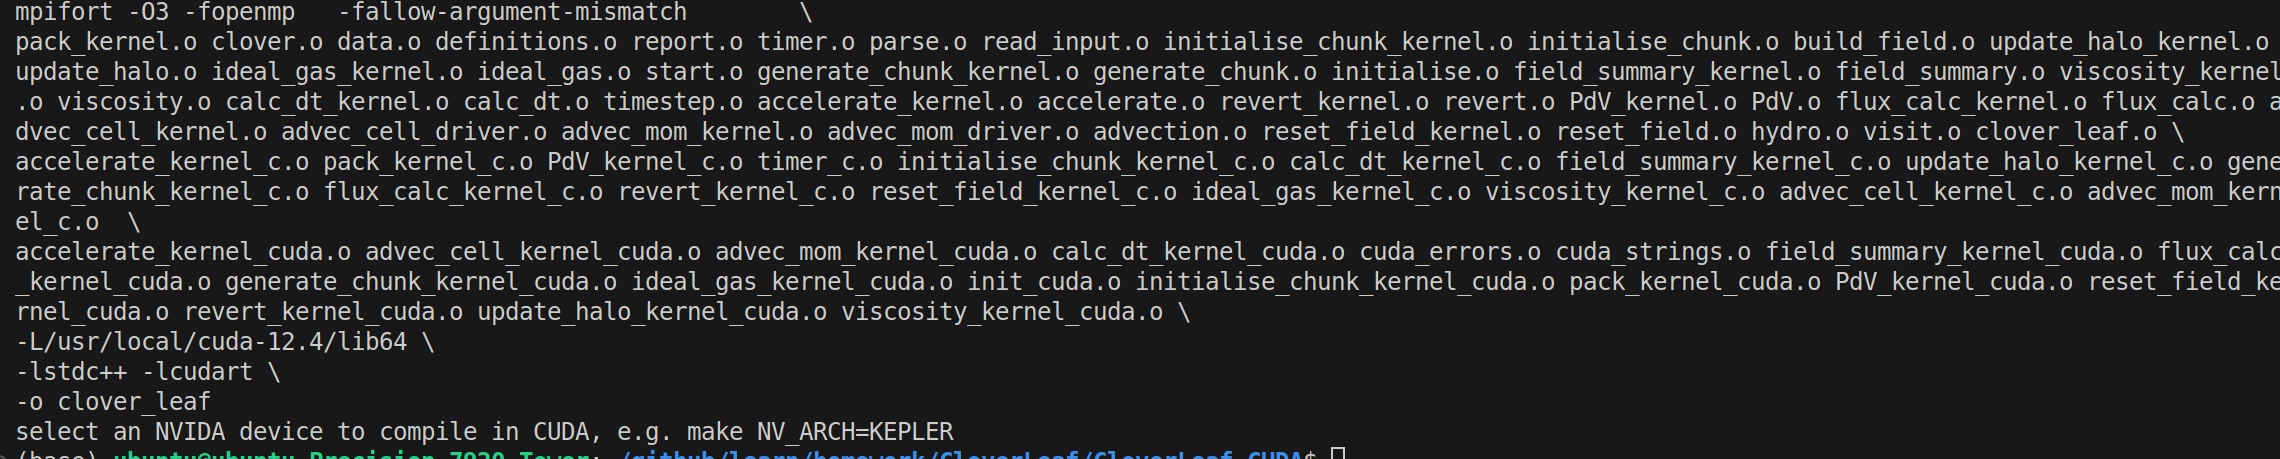
\includegraphics[width=0.8\textwidth]{./compile6.png}
    \caption{编译完成}
\end{figure}
测试结果,如下所示:
\begin{figure}[H]
    \centering
    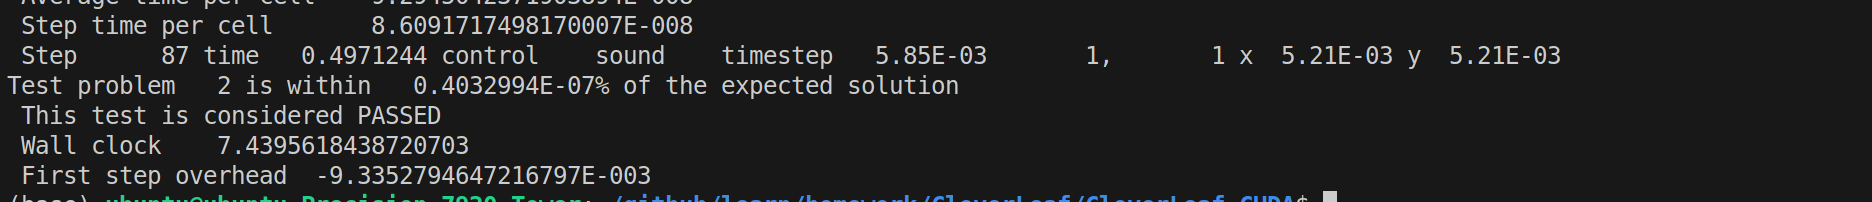
\includegraphics[width=0.8\textwidth]{./compile8.png}
    \caption{测试通过}
\end{figure}
\subsection{CUDA版本程序测试}
GPU=RTX 3090
CPU=gold 6132
Mpi\_num=1
openmp\_num=1
\begin{table}[h!]
    \centering
    \begin{tabular}{|c|c|c|}
    \hline
    \textbf{x\_cell} & \textbf{y\_cell} & \textbf{time consumption} \\
    \hline
    960 & 960 & 6.87124s \\
    \hline
    1920 & 960 & 22.105352s \\
    \hline
    3840 & 960 & 38.15225s \\
    \hline
    1920 & 1920 & 27.509817s \\
    \hline
    3840 & 1920 & 54.6727240s \\
    \hline
    3840 & 3840 & 114.67717s
    \end{tabular}
    \caption{CUDA 下不同网格大小的时间消耗}
    \label{table:combinations}
\end{table}
可以得出对比我的GPU和CPU,3090GPU约为15个左右的CPU加速效果
\subsection{CUDA代码技巧分析}
\end{CJK}
\end{document}